\documentclass[10pt,twocolumn,letterpaper]{article}

\usepackage{cvpr}
\usepackage{times}
\usepackage{epsfig}
\usepackage{graphicx}
\usepackage{amsmath}
\usepackage{amssymb}

% Include other packages here, before hyperref.

% If you comment hyperref and then uncomment it, you should delete
% egpaper.aux before re-running latex.  (Or just hit 'q' on the first latex
% run, let it finish, and you should be clear).
\usepackage[breaklinks=true,bookmarks=false]{hyperref}

\cvprfinalcopy % *** Uncomment this line for the final submission

\def\cvprPaperID{****} % *** Enter the CVPR Paper ID here
\def\httilde{\mbox{\tt\raisebox{-.5ex}{\symbol{126}}}}

% Pages are numbered in submission mode, and unnumbered in camera-ready
%\ifcvprfinal\pagestyle{empty}\fi
\setcounter{page}{4321}
\begin{document}

%%%%%%%%% TITLE
\title{\LaTeX\ Introduction}

\author{Mahmoud Ahmed\\
Arizona State University\\
Tempe, Arizona\\
{\tt\small meahmed@asu.edu}
}

\maketitle
%\thispagestyle{empty}

%%%%%%%%% ABSTRACT
\begin{abstract}
This paper introduces myself and my academic background using the CVPR
   format. Rather than presenting a research topic, we are to discuss 
   various aspects of my academic background and career objectives. 
   This paper also demonstrates how the structure of a conference paper 
   can be adapted for personal storytelling in an acedemic setting.
\end{abstract}

%%%%%%%%% BODY TEXT
\section{Introduction}
My name is Mahmoud Ahmed, and I am a computer science major 
at Arizona State University. My expertise spans both the theoretical 
and practical aspects of computer science. On the theoretical side, 
I have studied topics such as compiler construction, operating systems, 
data structures, and algorithms. On the practical side, 
I am experienced in programming with low-level languages such as C, 
as well as high-level languages such as Python, Javascript, and Java.

In addition to computer science, I possess a strong foundation in 
mathematics, including differential equations, linear algebra, and 
probability and statistics.


My current understanding of image analysis is still developing, 
and so far it has been limited to basic exposure to how image data is
 represented and manipulated. Nevertheless, I have always found it
  fascinating to explore how cutting-edge deep learning techniques can
   be applied to imaging, 
particularly in the context of medical diagnostics and healthcare.

%-------------------------------------------------------------------------
\subsection{Career objectives}
y career objective is to pursue research at the highest level 
and eventually become a doctoral student, with a 
particular focus on the fields of cryptography and statistical machine learning.

My interest in the aforementioned fields is driven not only by their
 practical impact in the real world but also by their mathematical 
 elegance and theoretical depth. I am particularly inspired by their 
 potential to improve human lives, especially in applications such as 
 computer vision and healthcare, where 
dvanced algorithms can support diagnostics, treatment, and overall wellbeing.

\subsection{Image processing demonstration}
For this demonstration, I processed a personal photograph using a standard camera,
and a processed version of the same photo.

\begin{figure}[h]
\centering

\includegraphics[width=0.17\textwidth]{p1n.jpeg}
\caption{Original image.}
\label{fig:processed_photo}
\end{figure}


\begin{figure}[h]
\centering
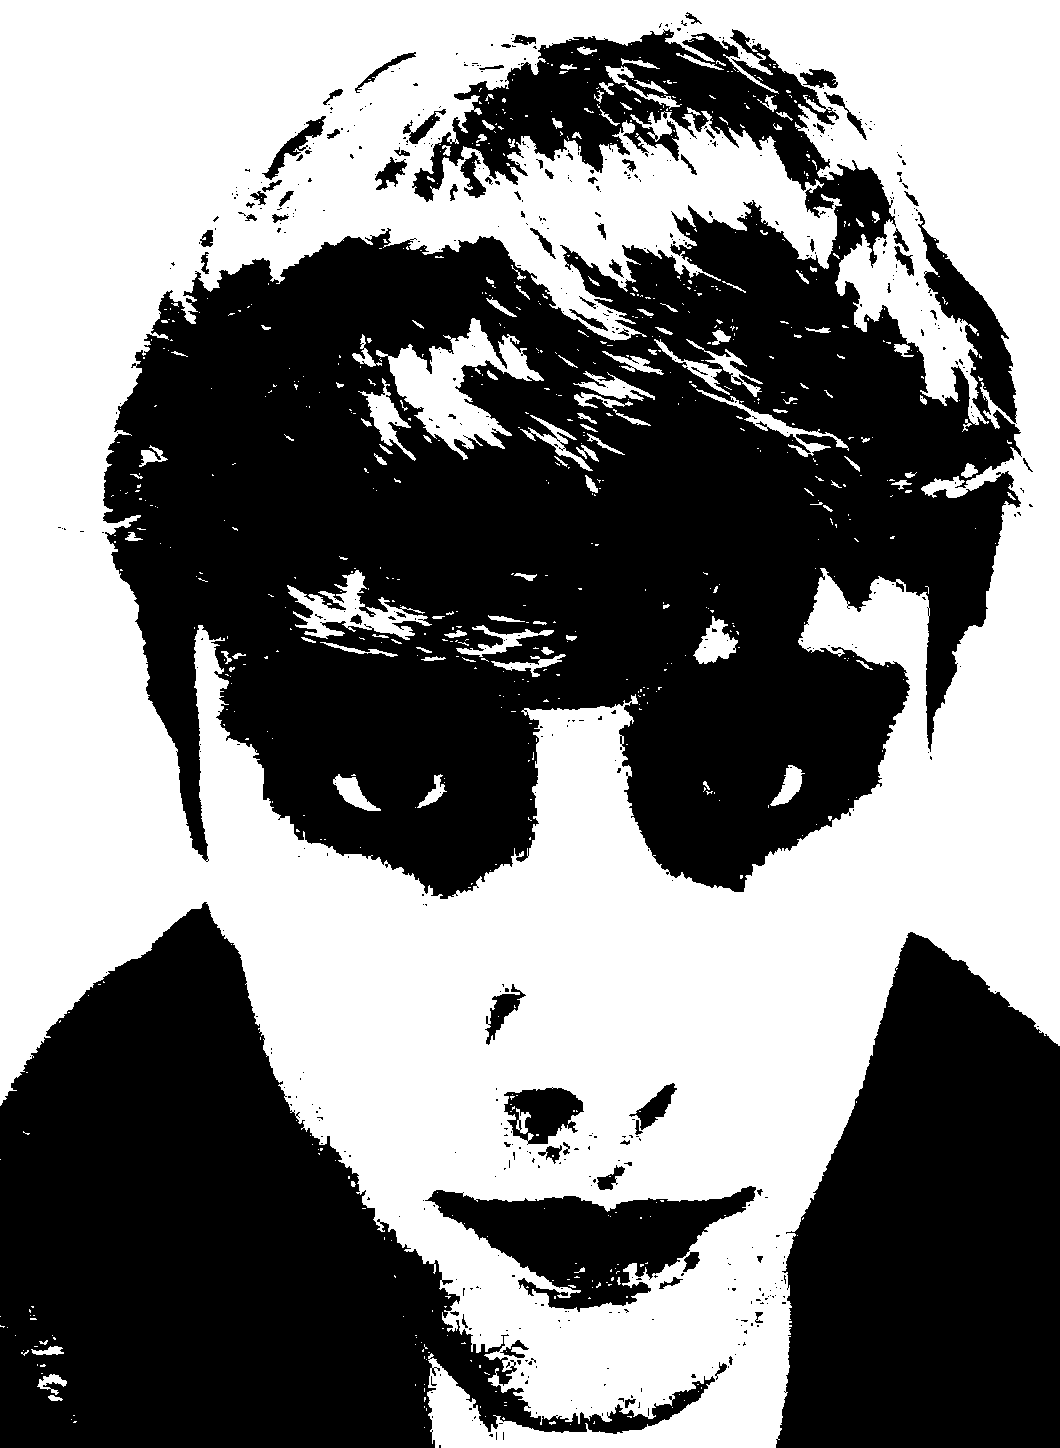
\includegraphics[width=0.17\textwidth]{pi.png}
\caption{Processed image after binary thresholding.}
\label{fig:processed_photo}
\end{figure}

The processed image was generated using a binary thresholding scheme \cite{opencv}
. 
In this approach, a threshold value is selected such 
that each pixel with an intensity above the threshold is 
assigned the maximum pixel value in the image, while all other 
pixels are set to zero. This operation converts the grayscale image
 into a binary image.
\[
\texttt{dst}(x,y) =
\begin{cases}
\texttt{maxval}, & \text{if } \texttt{src}(x,y) > \texttt{thresh} \\
0, & \text{otherwise}
\end{cases}
\]

where $\texttt{src}(x,y)$ is the intensity of the original image at
pixel $(x,y)$, $\texttt{thresh}$ is the threshold value chosen, and
$\texttt{maxval}$ is the maximum pixel value assigned to pixels above
the threshold.

The effect of this operation is to highlight bright regions of the
image while suppressing darker regions, effectively converting the
grayscale image into a binary image.

%-------------------------------------------------
\subsection{References}
\begin{thebibliography}{1}
\bibitem{opencv}
OpenCV, "OpenCV: Image Thresholding," Available: 
https://docs.opencv.org/4.x/d7/d4d/tutorial\_py\_thresholding.html [Accessed: Aug. 26, 2025].
\end{thebibliography}


\end{document}
